\chapter{Theory}
\label{chap:theory}
As the main principle of IDI is using intensity correlations of X-ray fluorescence, a basic recapitulation of the underlying definitions used in both simulations and the experimental application as well as (semi-) classical approach to coherence and the experiment of Hanbury-Brown Twiss will be given.


\section{X-Ray Fluorescence}
X-ray fluorescence is emitted if atoms are ionised leaving holes in the inner shells, which are subsequently filled by electrons of higher energy levels while the energy difference is emitted as photons, compared to the non-radiating Auger decay which is more likely for lighter atoms and/or L-shell excitation (see \fref{fig:levels} for the usual naming convention) \cite{santra2009}.  The finite lifetime of the excited states cause a predominantly Lorentzian line shape \cite{attwood1999,van2001}. In the experimental section, iron, copper and gallium atoms are considered - the relevant emission energies, the (experimental) line widths and relative intensities are shown in \fref{tab:elements}.   Roughly, the $K_\alpha$ line widths correspond to coherence times in the 0.4-0.8\,fs range \cite{krause1979}. The cross section for $K$-fluorescence is the highest just above the $K$-absorption edge and, for example for iron, an order of magnitude higher than the coherent cross section (see \fref{fig:cross}).

\begin{figure}
	\centering
	\begin{subfigure}[b]{0.35\textwidth}
		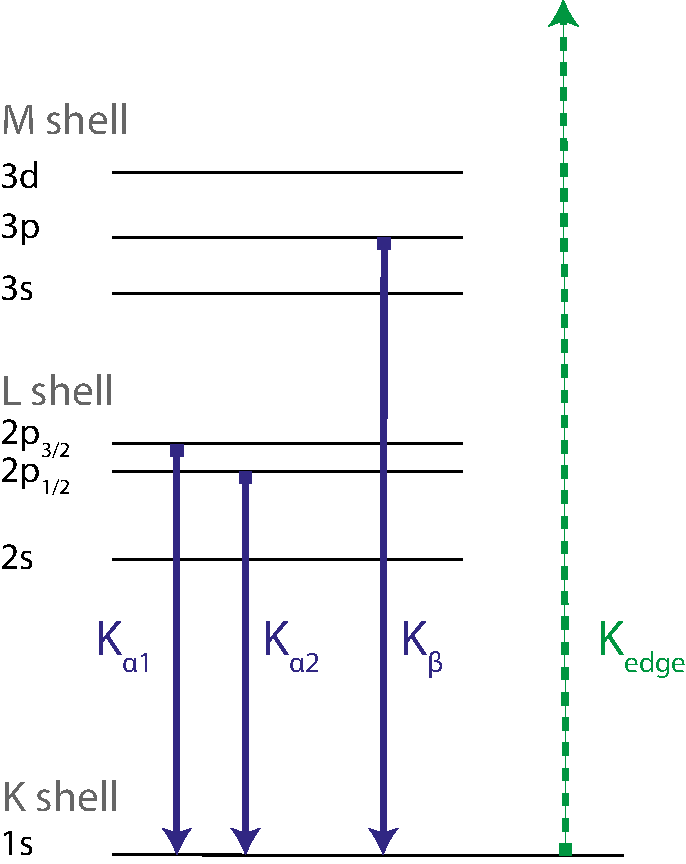
\includegraphics[width=\linewidth]{images/levels.pdf}
		\caption[Atomic Levels]{Atomic levels and associated X\nobreakdash-ray energies}
		\label{fig:levels}
	\end{subfigure}
	\begin{subfigure}[b]{0.45\textwidth}
		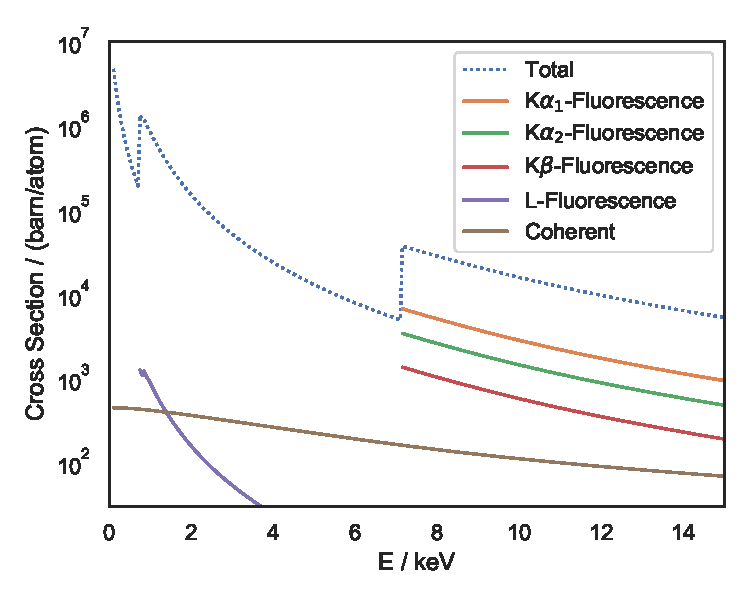
\includegraphics[width=\linewidth]{images/crosssectionFe.pdf}
		\caption[Cross Sections]{X-ray Cross Sections for Iron. Data from xraylib \cite{xraylib}}
		\label{fig:cross}
	\end{subfigure}
\end{figure}

\begin{table}
	\caption[X-ray Energies]{X-ray energies and line widths of some relevant elements \cite{xraylib,krause1979,sorum1987}.  }
	\label{tab:elements}
	\small
	\begin{tabular}{l|l|ll|lll|ll}
		\hline
		Element & K$_{edge}$                                             & \multicolumn{2}{c}{K$_{\alpha 1}$}                                                                           & \multicolumn{3}{c}{K$_{\alpha 2}$}                                                                                                                                       & \multicolumn{2}{c}{K$_{\beta}$}                                                                              \\
		& \begin{tabular}[c]{@{}l@{}}Energy \\ / eV\end{tabular} & \begin{tabular}[c]{@{}l@{}}Energy \\ / eV\end{tabular} & \begin{tabular}[c]{@{}l@{}}FWHM \\ / eV\end{tabular} & \begin{tabular}[c]{@{}l@{}}Energy\\  / eV\end{tabular} & \begin{tabular}[c]{@{}l@{}}FWHM \\ / eV\end{tabular} & \begin{tabular}[c]{@{}l@{}}rel. \\ Intensity\end{tabular} & \begin{tabular}[c]{@{}l@{}}Energy\\ / eV\end{tabular} & \begin{tabular}[c]{@{}l@{}}rel. \\ Intensity\end{tabular} \\ \hline
		Fe      & 7112                                                   & 6403.8                                                 & 1.61                                                 & 6390.8                                                 & 1.62                                                 & 0.50                                                      & 7058.0                                                & 0.17                                                      \\
		Cu      & 8979                                                   & 8047.8                                                & 2.11                                                 & 8,027.8                                                & 2.17                                                 & 0.51                                                      & 8905.3                                                & 0.17                                                      \\
		Ga      & 10367                                                  & 9251.7                                                 & 2.59                                                 & 9224.8                                                 & 2.66                                                 & 0.51                                                      & 10263.9                                               & 0.18                                                      \\
		As      & 11867                                                  & 10543.7                                                & 3.08                                                 & 10508.0                                                & 3.17                                                 & 0.51                                                      & 11724.3                                               & 0.19                                                      \\ \hline
	\end{tabular}
\end{table}

\section{Basic Concepts of Coherence}
In the following, for simplicity, all considered fields are initially assumed to be both stationary and ergodic: A process $f(t)$ is wide-sense stationary, if the expectation value $E[f(t)]$ is independent of the time $t$ and $E[f(t_1)f(t_2)]$ depends only on the time difference $\tau=f_1-f_2$. A process, for which the time average and the ensemble average are equal is called ergodic. Stationarity is a necessity for ergodicity \cite{goodman2000}. It can be shown, that the basic principles hold for non-stationary fields with the main difference being, that all expectation values have to be taken over different realizations \cite{lajunen04}.

Spherical waves as solutions wave equation in spherical coordinates,
\begin{equation}
	\vec{E}(\vec{r},t)=\vec{E}_0(k,t) \frac{e^{i\vec{r}\vec{k}-iwt}}{R}
	\end{equation}
describe the electric field of light propagating isotropically in vacuum. 
The superposition principle allows the addition of two waves (with the real amplitudes $\vec{A}_{1,2}$ and phases $\phi_{1,2}$)
\begin{equation}
\vec{E}(\vec{r},t)=\vec{E_1}(\vec{r},t)+\vec{E_2}(\vec{r},t)=\vec{A_1}*e^{i\phi_1} * e^{i\vec{r}\vec{k_1}-iw_1t} + \vec{A_1}*e^{i\phi_1} * e^{i\vec{r}\vec{k_2}-iw_2t} 
\end{equation} 
The measured intensity with measurement time $T$ will be
\begin{equation}
	I(\vec{r},t)\propto \frac{1}{T} \int_0^T \left|E(\vec{r},t)\right|^2 \diff t
	\stackrel{T\gg1/w}{\propto}
    \left<\left|E(\vec{r},t)\right|^2\right> \,.
\end{equation}

The superposition of two monochromatic, stationary waves with a fixed phase difference $\Delta \phi$, such as a wave and its time delayed copy (\fref{fig:michelson}) in an interferometer, gives rise to interference fringes
\begin{align}
	\left<I(\vec{r},t)\right> & = I_1+I_2+2\left<\Re({E_1(\vec{r},t)}E_2^*(\vec{r},t))\right> \\
	& = I_1+I_2+2\sqrt{I_1I_2}\cos\left((\vec{k_1}-\vec{k_2})\vec{r}+\Delta \phi\right) 
\label{eq:interference}
\end{align}

Defining the contrast of the fringes as the visibility $V$,
\begin{equation}
	V=\frac{I_{max}-I_{min}}{I_{max}+I_{min}} ,
\end{equation} 

results for equal intensities of the the waves in maximum contrast,  $V=\frac{2\sqrt{I*I}}{I+I}I=1$. This case of a fixed phase difference is called \textit{coherent}.
If, on the other hand, the phase difference $\Delta \phi$ is not fixed but completely random and therefore averages out in \fref{eq:interference}, the visibility goes to 0 and the waves are regarded as \textit{incoherent}  \cite{born1980,goodman2000}

To consider non monochromatic waves, we define the self coherence function $\Gamma$ as 
\begin{equation}
\Gamma(\tau)=\left< E(t)E(t+\tau)\right>
\end{equation}
and its normalized version, the complex degree of (self-)coherence $\gamma$, as
\begin{equation}
\gamma(\tau)=\frac{\Gamma(\tau)}{\Gamma(0)} =  \frac{\Gamma(\tau)}{<I>}
\end{equation} 
Now \fref{eq:interference} can be written as 
\begin{equation}
	I=I_{1}+I_{2}+2 \sqrt{I_{1} I_{2}} \operatorname{Re}\left[\gamma(\tau)\right]
\end{equation}
and (again for equal intensities) the visibility is $V(\tau)=\left|\gamma(\tau)\right|$ \cite{zernike1938,loudon2000}.

The \textit{coherence time }shall describe at which delay the visibility falls to approximately zero. One possible definition by Mandel based on the complex degree of coherence,
\begin{equation}
\tau_c = \int_{-\infty}^{\infty} \left| \gamma(\tau)\right|^2 \diff \tau 
\end{equation} will be used in the following. Other definitions commonly used are equivalent up to a constant factor and lead generally to coherence times of the same order of magnitude \cite{mandel1959,goodman2000}. 

The Wiener Khinchin theorem connects the power spectrum $F(w)$ with $\gamma$ \cite{goodman2000,lajunen04}.
\begin{equation}
	F(\omega)=\frac{1}{2 \pi} \int_{-\infty}^{\infty} \gamma(\tau) \exp (\mathrm{i} \omega \tau)  \dif \tau \,.
\end{equation}.

As a relevant example, for an exponentially decaying electric field envelope\footnote{Corresponding to an intensity/photon number decay with time constant $\sfrac{\tau}{2}$} $E(t)=\Theta(t)e^{-t/\tau_E}$, the power spectrum is Lorentzian with an angular frequency FWHM of $\Delta \omega=\frac{2}{\tau_E}$,
\begin{equation*}
\left|\int_{0}^{\infty}  e^{-t/\tau_E} e^{-iwt} \dif t \right|^2 \propto  \frac{1}{1/\tau_E^2+w^2} .
\end{equation*}
and
\begin{align*}
\left\langle E(t) E^{*}(t+\tau)\right\rangle
&=\int_{0}^{\infty} E(t) E^{*}(t+\tau)\diff t
=\frac{\tau_E}{2}   e^{-\frac{\left| \tau \right| }{\tau_E }}\\
\left\langle E(t) E^{*}(t)\right\rangle
&=\frac{\tau_E}{2} 
\end{align*}
Hence, $\left<\gamma(\tau)\right>=e^{-|\tau/| \tau_E}$,   and the coherence time as defined is above is $\tau_c=\int_{-\infty}^{\infty} \left| \gamma(\tau)\right|^2 \diff \tau=\tau_E=\sfrac{2\hbar}{\Delta E}$ \cite{goodman2000,pollnau2020}.



 \begin{figure}
	\centering
	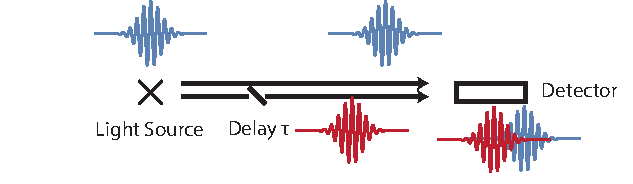
\includegraphics[width=0.8\linewidth]{images/michelson.pdf}
	\caption[Schematic of interferometer]{Schematic of interferometer: Light of (a Gaussian) light source with finite coherence time is split and interference with a delayed copy is observed. The time averaged intensity measured by an detector changes with the delay time. }
	\label{fig:michelson}
\end{figure}


\paragraph{First order coherence $g^1$}
A generalization of $\gamma$  to different fields  $E_1^*(\vec{r}_1,t_1)$ and $E_2(\vec{r}_2,t_2)$ is the normalized first order correlation function $g^1$ \cite{agarwal2013}
\begin{equation}
	g^{(1)}(\vec{r}_1,t_1;\vec{r}_2,t_2)= \frac
	{\left< E_1^*(\vec{r}_1,t_1)E_2(\vec{r}_2,t_2) \right>}
	{\left[ \left<\left | E(\vec{r}_1,t_1)\right |^2 \right> \left< \left |E(\vec{r}_2,t_2)\right |^2 \right>\right]^{1/2}}	\,.
\end{equation}



This can be used for example to describe Young's double slit experiment (\fref{fig:doubleslit}): On the screen at point $\vec{r}$, the electrical field is 
\begin{equation}
	E(\vec{r}, t)=\frac{E\left(\vec{r}_{1}, t-R_{1} / c\right)}{R_{1}} e^{i\left[\vec{k}_{1} \cdot\left(\vec{r}-\vec{r}_{1}\right)-\omega t\right]}+\frac{E\left(\vec{r}_{2}, t-R_{2} / c\right)}{R_{2}} e^{i\left[\vec{k}_{2} \cdot\left(\vec{r}-\vec{r}_{2}\right)-\omega t\right]} \,.
\end{equation}
If the distances from $r$ to the two slits are (approximately) equal, $R_{1}\approx R_{2} \approx d$, the intensity at $\vec{r}$ is
\begin{align*}
	\left\langle I_{P}\left(\vec{r}, t^{\prime}\right)\right\rangle&=\left\langle\left|E\left(\vec{r}_{1}, t\right)\right|^{2}\right\rangle+\left\langle\left|E\left(\vec{r}_{2}, t\right)\right|^{2}\right\rangle 
	+\left[\left\langle E^{*}\left(\vec{r}_{1}, t\right) E\left(\vec{r}_{2}, t\right)\right\rangle e^{i\left(\vec{k}_{1}-\vec{k}_{2}\right) \cdot \vec{r}+i \Delta \phi}+\text{c.c}\right] \\
	& \propto 1+
	\frac{2 \sqrt{\left< I\left(\vec{r}_{1}, t\right)\right>\left< I\left(\vec{r}_{2}, t\right)\right>}}
	{\vphantom{2\sqrt{\left<I\left(\vec{r}_{1}\right)\right>}}\left< I\left(\vec{r}_{1}, t\right)\right>+\left< I\left(\vec{r}_{2}, t\right)\right>}	
	\frac{\vphantom{2\sqrt{\left<I\left(\vec{r}_{1}\right)\right>}}\left< E^{*}\left(\vec{r}_{1}, t\right) E\left(\vec{r}_{2}, t\right)\right>}
	{\vphantom{2\sqrt{\left<I\left(\vec{r}_{1}\right)\right>}}\sqrt{\left\langle I\left(\vec{r}_{1}, t\right)\right>\left\langle I\left(\vec{r}_{2}, t\right)\right>}}
	\cos \left[\left(\vec{k}_{1}-\vec{k}_{2}\right) \cdot \vec{r}+\Delta \phi\right]
\end{align*}


and the visibility can be identified as the modulus of $g^1$ \cite{loudon2000,ou2017}.

\begin{figure}
	\centering
	\begin{subfigure}[b]{0.53\textwidth}
	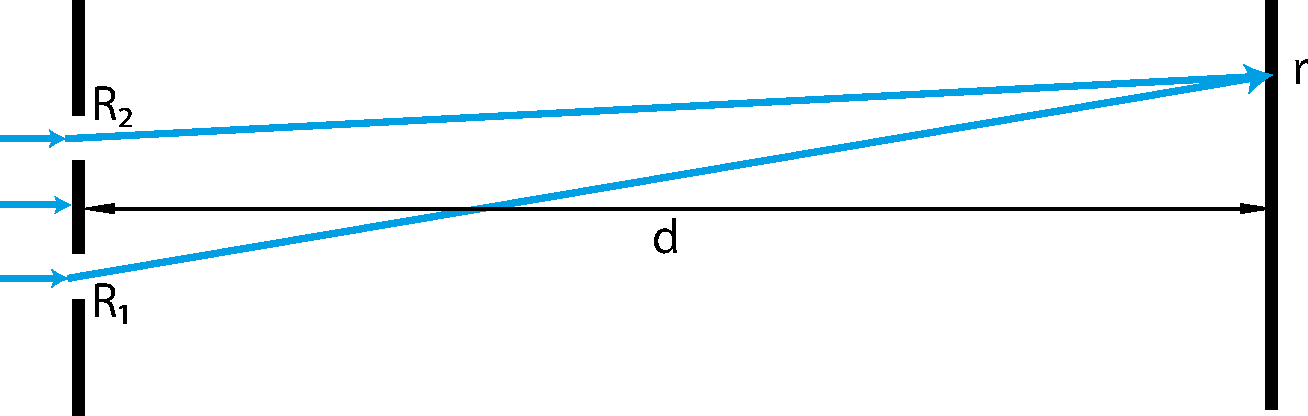
\includegraphics[width=\linewidth]{images/doubleslit.pdf}
	\caption[Schematic of a lit]{Schematic of a double slit.}
	\label{fig:doubleslit}
	\end{subfigure}
\begin{subfigure}[b]{0.41\textwidth}
	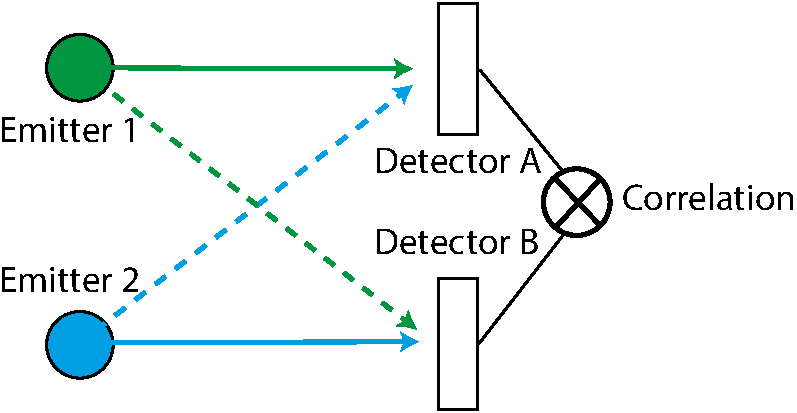
\includegraphics[width=\linewidth]{images/correlation.pdf}
	\caption{Two photon interference in HBT.}
	\label{fig:twophoton}
\end{subfigure}
\caption[Schematic of double slit and two photon interference in  HBT experiments]{\textbf{(a)} Monochromatic light goes through slits located at $R_1$ and $R_2$. The intensity at a position $r$ on the scree (in distance $d$) is the superposition of both paths.  If the slits are within the lateral coherence area of the source, the visibility of the interference pattern depends on the path length difference in comparison to the coherence time $\tau$.
In the Hanbury Brown Twiss experiment\textbf{(b)} are two indistinguishable two photon states, illustrated as dashed and  continuous lines respectively: Either simultaneously a photon from emitter 1 is detected by detector A and from emitter 2 by detector B or from emitter 1 by detector B and from emitter 2 by detector A.}
\end{figure}



\paragraph{Second order coherence $g^2$}
The definition of $g^1$ can be extended to the second order by considering
\begin{equation*}
	g^{(2)}(\vec{r}_1,t_1;\vec{r}_2,t_2)= 
	\frac{\left< E^*(\vec{r}_1,t_1)E^*(\vec{r}_2,t_2)E(\vec{r}_1,t_1)E(\vec{r}_2,t_2) \right>}{\left<\left | E(\vec{r}_1,t_1)\right |^2 \right> \left< \left |E(\vec{r}_2,t_2)\right |^2 \right>}	
\end{equation*}
For classical fields, this is equivalent  to normalized correlations of intensities \cite{goodman2000}:
\begin{equation}
	g^{(2)}(\vec{r}_1,t_1;\vec{r}_2,t_2)= 
		\frac{\left< I(\vec{r}_1,t_1)I(\vec{r}_2,t_2 \right>}{\left<I(\vec{r}_1,t_1)\right>\left<I(\vec{r}_2,t_2)\right>}	
		\label{eq:g2}
\end{equation}


\paragraph{Van Cittert Zernicke}
The Van Cittert–Zernike theorem establishes that in the far field, the coherence function of a 
quasi-monochromatic but spatially incoherent light source is proportional to the 2D Fourier transform intensity distribution of the source. Carter and Wolf introduced a generalization for three dimensional sources (without the need for a small angle approximation), showing that in the case of an completely incoherent source field, the first order coherence in the far field is proportional to the 3D Fourier transform of the source's intensity distribution \cite{rosen1996, goodman2005, carter1981}:
\begin{equation}
	g^{(1)}(\vec{r}_1,\vec{r}_2) \propto I_0^{-1} \int_{S} I_s(\vec{r}) e^{ik(R_1-R_2)} \difc \vec{r} \approx I_0^{-1} \int_{S} I_s(\vec{r}) e^{-ik\vec{r}(\vec{r_1}-\vec{r_2})} \difc \vec{r}
	\label{eq:vcz}
\end{equation}
with the source volume $S$ and intensity distribution $I_s$, total source intensity $I_0=\int I_s(\vec{r}) \difc \vec{r}$ and distances $R_{1,2}=\left|\vec{r}_{1,2}-\vec{r}\right|$.
%-Hanbury Brown and Twist


%-Single Photon Emitters/2nd Quant description
%(siehe Referenzen in Schaller/resonance fluorescence)
%-Fluorescence g2
%$2 Level with finite Lifetime -> Spectrum of fluorescence
%\section{X-Ray Fluorescence}


\section{Hanbury Brown Twiss}
Hanbury-Brown Twiss first used the correlation between the intensities captures by photomultiplier tubes to measure the angular size of stars  \cite{hanbury1956}. The underlying effect can be explained based on (semi-)classical coherence theory for chaotic light sources \cite{baym1997,goodman2000}:

If the sources $A$ and $B$ (in the original experiment different parts of the observed star) produce each spherical electromagnetic waves with random but constant phases $\phi_{A,B}$, $E_{A,B}=c_{A,B} e^{i k\left|\vec{r}-\vec{r}_{1,2}\right|+i \phi_{A,B}} /\left|\vec{r}-\vec{r}_{A,B}\right|$ and ignoring polarization, the total intensity $I_{1}$ at detector 1 (and similar at detector 2) is
\begin{equation}
	I_{1} =
	\frac{1}{L^{2}}\left(
	|c_A|^{2}
	+|c_B|^{2}
	+c_A^{*} c_B     e^{ i\left(k\left(r_{1 b}-r_{1 a}\right)+\phi_{B}-\phi_{A}\right)}
	+c_A     c_B^{*} e^{-i\left(k\left(r_{1 b}-r_{1 a}\right)+\phi_{B}-\phi_{A}\right)}
	\right)
\end{equation}
with $r_{1 a}$ the distance from source $A$ to detector 1 etc. 
Averaging over many independent realizations of the random phases leads to the average intensities in the two detectors,
\begin{equation}
	\left\langle I_{1}\right\rangle=\left\langle I_{2}\right\rangle=\frac{1}{L^{2}}\left(\left\langle|c_A|^{2}\right\rangle+\left\langle|c_B|^{2}\right\rangle\right)
\end{equation}, 

independent of the separation of the detectors. On the other hand, the average of the product of the intensities is
\begin{equation}
	\left\langle I_{1} I_{2}\right\rangle =
	\left\langle I_{1}\right\rangle\left\langle I_{2}\right\rangle+\frac{2}{L^{4}}|c_A|^{2}|c_B|^{2} \cos \left(k\left(r_{1 a}-r_{2 a}-r_{1 b}+r_{2 b}\right)\right) 
\end{equation}.
Hence,
\begin{equation}
	\frac{\left\langle I_{1} I_{2}\right\rangle}{\left\langle I_{1}\right\rangle\left\langle I_{2}\right\rangle}
	=1+2 \frac{\left\langle|\alpha|^{2}\right\rangle\left\langle|\beta|^{2}\right\rangle}{\left(\left\langle|\alpha|^{2}\right\rangle+\left\langle|\beta|^{2}\right\rangle\right)^{2}} \cos \left(k\left(r_{1 a}-r_{2 a}-r_{1 b}+r_{2 b}\right)\right)
\end{equation}

For a large enough separation between the sources and detectors $(L \gg R)$, the small angle approximation can be made and
\begin{equation}
	g^2\left(\vec{k_1}-\vec{k_2}\right)-1\propto \cos{\left(\vec{R} \cdot\left(\vec{k}_{2}-\vec{k}_{1}\right)\right)}
\end{equation} 
where $\vec{k}_{1,2}=k \vec{r}_{1,2}$ is the wavevector of the light seen in detector $1$/detector $2$. As the modulation frequency of the the intensity correlation is depended $R$, the separation of the two sources (the size of the star) can be recovered.

A more detailed quantum mechanical treatment considers the mixtures of the probability amplitudes of emission and detection at the two detectors (as the individual paths are indistinguishable), leading what was shown as an equivalent description of the HBT effect for thermal light sources \cite{fano1961,sudarshan1963,glauber2006}, but allows the treatment of non classical light sources such as single photon emitters \cite{mandel1995,classen2017}. This introduces a correction term in $g^2$ of the order of $1/N$ with $N$ the number of emitters, which for the considered cases is negligible.



\paragraph{Siegert Relation}
For chaotic light with Gaussian statistics, Isserlis' theorem 
$\left<ABCD\right>=\left<AB\right>\left<CD\right>+\left<AC\right>\left<BD\right>+\left<AD\right>\left<BC\right>$ can be applied to \fref{eq:g2}, leading  (independently of the spatial configuration of the sources ) to
\begin{equation}
	g^2(\vec{r_1},\vec{r_2}) = 1+ |g^1(\vec{r_1},\vec{r_2}) |^2 ,
\end{equation}
which is called the Siegert Relation \cite{ou2017}.
For $N$ Single-Photon-Emitters and quantum optical treatment,  a similiar form holds \cite{classen2017}:
\begin{equation}
	g^2(\vec{r_1},\vec{r_2}) = 1+ |g^1(\vec{r_1},\vec{r_2}) |^2 - \frac{2}{N} ,
\end{equation}
As, as according to the van Cittert Zernicke theorem (\fref{eq:vcz}), $g^1$ encodes structural information, 
\begin{equation}
	g^1(\vec{k_1},\vec{k_2}) \propto \mathscr{F}S(\vec{r}) = S(\vec{q})
\end{equation}
the difference of the intensity-intensity correlation from unity is proportional (with a contrast determining constant $\beta$) to the Fourier transform of the arrangement of emitters with $q=\vec{k_1}-\vec{k_2}$ (see \fref{fig:scatteringvectors}).
This is the basic principle used in IDI to recover three dimensional spatial information from the intensity correlation.
\begin{figure}
	\centering
	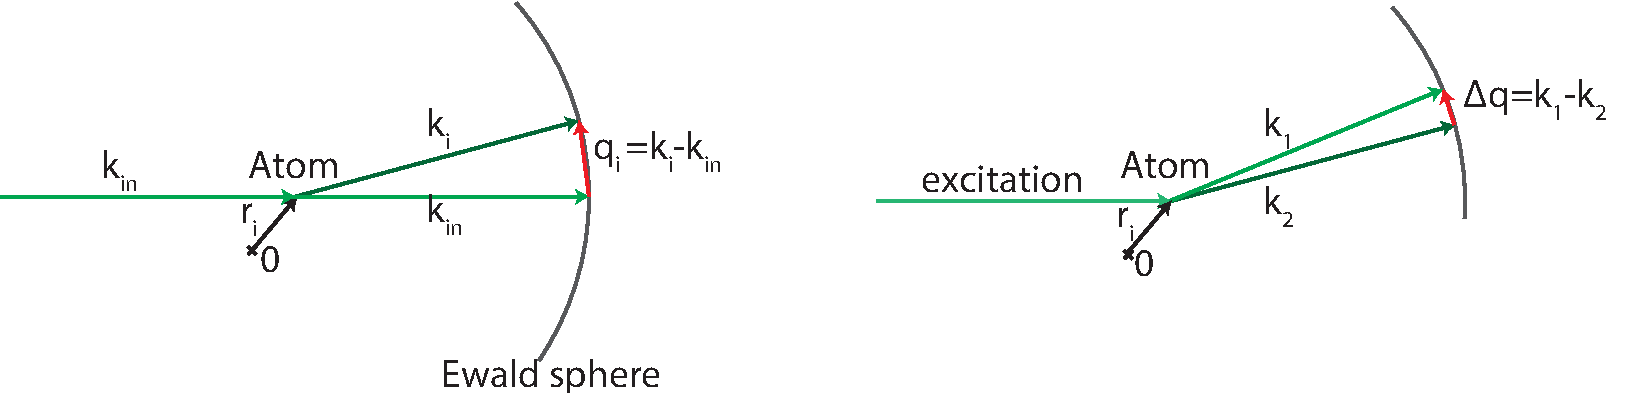
\includegraphics[width=0.9\linewidth]{images/scatteringvectors.pdf}
	\caption[Scattering Vectors]{Scattering vector $q$ in CDI (left) and IDI (right). In CDI, $q$ is the momentum transfer between incoming and outgoing wave. In IDI, there is no momentum transfer from the incoming to the outgoing wave. Instead, intensity correlations of different $k_1$, $k_2$ give a momentum transfer $\delta q$ according to the Siegert relation.}
	\label{fig:scatteringvectors}
	
\end{figure}

\section{Photon Statistics}
Considering a complex sum of many phasors (e.g. the superposition of many electrical fields or probability amplitudes) of constant amplitude $A$ and independent uniformly in $(-\pi,\pi]$ distributed phases $\phi_k$,
\begin{align}
	c=\sum^N_k A e^{i\phi_k}
\end{align}
for sufficiently large numbers of $N$, the real and imaginary parts
\begin{align*}
	r&=\Re c =  A \sum^N_k \cos(\phi_k) &
	i&= \Im c =A \sum^N_k \sin(\phi_k)
\end{align*}
will (by Central Limit Theorem) be Gaussian random variables with zero mean and variance $\sigma^2=\frac{N}{2}A^2$, the probability distribution of the amplitude $a=\sqrt(a^2+i^2)$ will therefor be the Rayleigh distribution
\begin{equation}
	p(a)=\frac{1}{2\pi\sigma^2} a e^{\frac{a^2}{2\sigma^2}}
\end{equation}
and  $I=\left|a\right|^2$ will  follow an exponential distribution
\begin{equation}
	\label{eq:expdistr}
	p(I)=\frac{ e^{-I/\overline{I}}}{\overline{I}}
\end{equation} 
with mean $\overline{I}$ and standard deviation $\sigma=\overline{I}$  \cite{goodman2000,goodman1976}.
A sum of $M$ uncorrelated random variables following identical distributions given by \fref{eq:expdistr} follows a Gamma distribution,
\begin{equation}
	\label{eq:gammadistr}
	p(I)=\frac{I^{M-1} e^{-I/\overline{I}}} {\overline{I}^M \Gamma(M)}.
\end{equation}
For a positive integer $M$ this simplifies with $\Gamma(M)=(M-1)!$ to an Erlang distribution  \cite{forbes2010,trost2020}.
If $I$ is distributed like \fref{eq:gammadistr} and furthermore Poisson sampled as discrete $k$ (such as photon counts in the semi-classical picture), it is negative binomial distributed,
\cite{trost2020,mandel1959,holmes2019}
\begin{equation}
	p(k)=
	\frac{\Gamma(k+M)}{\Gamma(M)\Gamma(k+1) }
	\left( 1+\frac{1}{\overline{I}}
	\right)^{-k}
	\left( 1+\overline{I}
	\right)^{-M}
	\label{eq:negbinomialdist}
\end{equation}
with mean $\mu=M\overline{I}$ and variance $\mu+\frac{\mu^2}{M}$ (which is higher than the variance of the Poisson distribution $\mu$ ).

This probability distribution can be compared to an experimental measured photon count distribution and the number of modes present in the measurement can be estimated by a regression for small mode numbers \cite{lehmkuhler2014,yun2019}. 
For low photon numbers, a simplified approach can be used by only considering single- and two-photon events: By considering the ratio of the probabilities of those events, $p(1) / p(2)$,  an expression for the number of modes can be found, which can be simplified with a low intensity approximation $\mu\approx p(1)+2p(2)+O(\mu^2)$ to 
\begin{equation}
	M=\frac{\mu  (p(1)-2 p(2))}{2 p(2)-\mu  p(1)}\approx \frac{p(1)^2}{2 p(2) (1-p(1))-p(1)^2}
	\label{eq:modesp1p2}
\end{equation}
as an estimation for the number of modes.
If $p(1)$ and $p(2)$ are estimated as $p'_1$ and $p'_2$ based on the frequency in experimental observations, the uncertainty of the mode estimate can be estimated as 
$\Delta M \lesssim \frac{2 p'_1}{\left({p'_1}^2+2 (p'_1-1) p'_2\right)^2} \left(\Delta p'_1 (2-p'_1) p'_2+\Delta p'_2 (1-p'_1) p'_1\right)$.


\section{Signal to Noise Considerations}
\label{sec:specklecontrast}
The Signal to Noise characteristics of the method are determined by the noise and the signal:
The signal strength is determined by $\left|S(q)\right|^2$, which is dependent and the sample, and the contrast of the recorded speckle image. The noise in the measurement will consist of three parts: First, noise inherent to IDI caused by the random distribution of phases, second, the poissonian noise caused by quantized photons, and third, experimental noise \cite{trost2020, goodman2007}. 

\paragraph{Speckle Contrast}

The speckle contrast $\beta =\tfrac{1}{M}$ is governed by the number of independent modes $M$ overlaid in the measurement \cite{goodman2000}. 
If the measurement is performed over a finite amount of time, the number of temporal modes is
\begin{equation}
M_t=\frac{\left(\int_{-\infty}^{\infty} P(t)\diff t\right)^2}{\int_{-\infty}^{\infty} K(t) \left|\mu(t)\right|^2\diff t}
\label{eq:modes}
\end{equation}
with $P(t)$ the integration window weighting function and $K(t)$ its autocorrelation \cite{goodman2007}. If the integration windows is set by the integration time $T$ of the detector, $P(t)$ is a rectangular function with the width $T$ and
\begin{align}
M_{t,\text{rect}} =T \left[\int_{-\infty}^{\infty} \Lambda\left(\frac{t}{T}\right) \left|\mu(t)\right|^2 \diff t \right]^{-1} .\\
\text{with  }\Lambda(x) = \begin{cases} 
 1-\left|x\right|& \textit{if }|x|<1\\
0 & \textit{otherwise}\\ 
\end{cases}
\label{eq:modesapprox}
\end{align}
Considering the case of a long integration time, $T\gg\tau$, this can be approximated as $M\approx\frac{T}{\tau}$. For a short integration time,  $T\ll\tau$, the number of temporal modes $M$ approaches unity.

If the Integration time can be considered as infinite and instead $P(t)$ is a Gaussian excitation pulse with FWHM of $2\sigma\sqrt{2\ln2}$, creating to a non-stationary field, this leads to
\begin{equation}
	M_{t,\text{Gauss}}=e^{\frac{4 \sigma ^2}{\tau ^2}} \text{erfc}\left(\frac{2 \sigma }{\tau }\right),
	\label{eq:mgauss}
\end{equation}
with the complementary error function $\erfc=\frac{2}{\sqrt{\pi}}\int_x^\infty e^{-z^2}\diff z$.

Inoue et al. considered $P$ to be the Gaussian excitation pulse convoluted with an exponential decay with lifetime $\tau$ \cite{inoue2019,butz2015},
\begin{align}
P(t)&=\frac{1}{\tau\sigma\sqrt{2\pi}} \int_0^{\infty} e^{-\frac{t^{\prime}}{\tau}} 
e^{-\frac{(t-t^{\prime})^2}{2\sigma^2}}\diff t^{\prime}
=\frac{1}{2\tau}e^{-\frac{t}{\tau}+\frac{\sigma^2}{2\tau^2}}
\erfc\left[
\frac{\sigma}{\sqrt{2}\tau}
-\frac{t}{\sqrt{2}\sigma}
	\right] ,
	\label{eq:pfull}
	\end{align}
	An approximation can be made if the pulse length is long in comparison to the coherence time, simplifying the auto-correlation of $P$ to
\begin{align}
K(t)&=\int_{-\infty}^\infty \frac{1}{4
	\tau ^2}e^{-\frac{t^2}{2 \sigma ^2}-\frac{(t+t')^2}{2 \sigma ^2}}
\erfcx\left(\frac{\sigma^2 -t \tau }{\sqrt{2} \tau \sigma}\right)
\erfcx\left(\frac{\sigma^2 -\tau  (t+t')}{\sqrt{2} \tau \sigma }\right) \diff t' \nonumber \\
&\stackrel{\tau \rightarrow 0}{\approx} \frac{1}{2\sqrt{\pi}\sigma} e^{-\left(\frac{t}{2\sigma}\right)^2} 
\label{eq:kapprox}
\end{align}
with the scaled complementary error function\footnote{To numerically evaluate \fref{eq:mgauss}, \fref{eq:pfull} and integrals involving them, the introduction of the scaled complementary error function and switching to a sufficient approximation is beneficial to avoid under- or overflow of the numerical representation of either the exponential or the error function term.} $\erfcx(x)=e^{x^2}\erfc(x)\stackrel{x\gg1}{\approx}  \frac{1}{\sqrt{\pi}x}$
   \cite{ren2007}.
The number of degrees of freedom, $M_{t,\text{Conv}}=\left[\int_{-\infty}^{\infty} K(t) \left|\mu(t)\right|^2\diff t\right]^{-1}$  can then be numerically evaluated  for a Lorentzian spectrum as shown in \fref{fig:theorymodes}.

\begin{figure}
	\centering
	\begin{subfigure}[b]{0.48\textwidth}
		\centering
		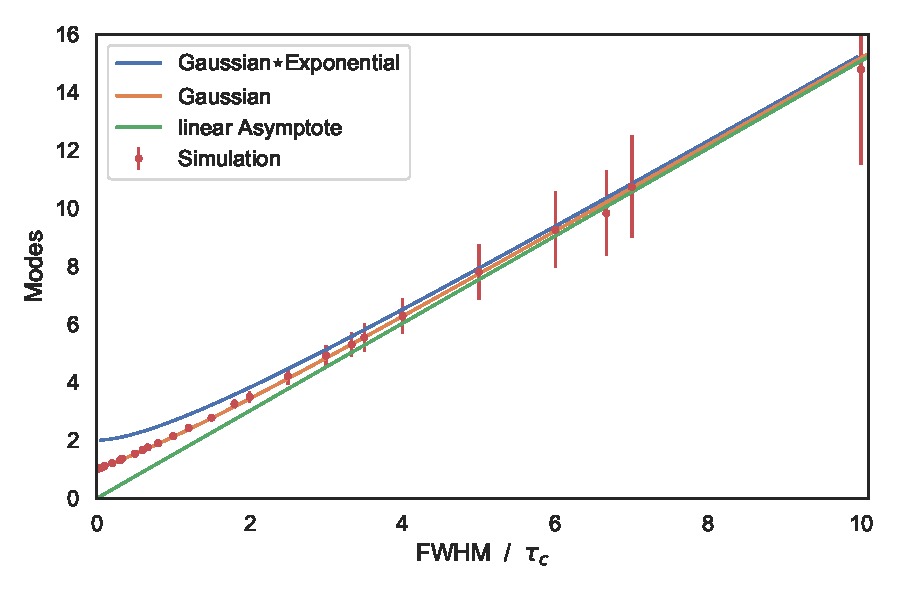
\includegraphics[width=\linewidth]{images/temporalmodes.pdf}
		\caption{Temporal Modes}
		\label{fig:theorymodes}
	\end{subfigure}
	\begin{subfigure}[b]{0.48\textwidth}
		\centering
    	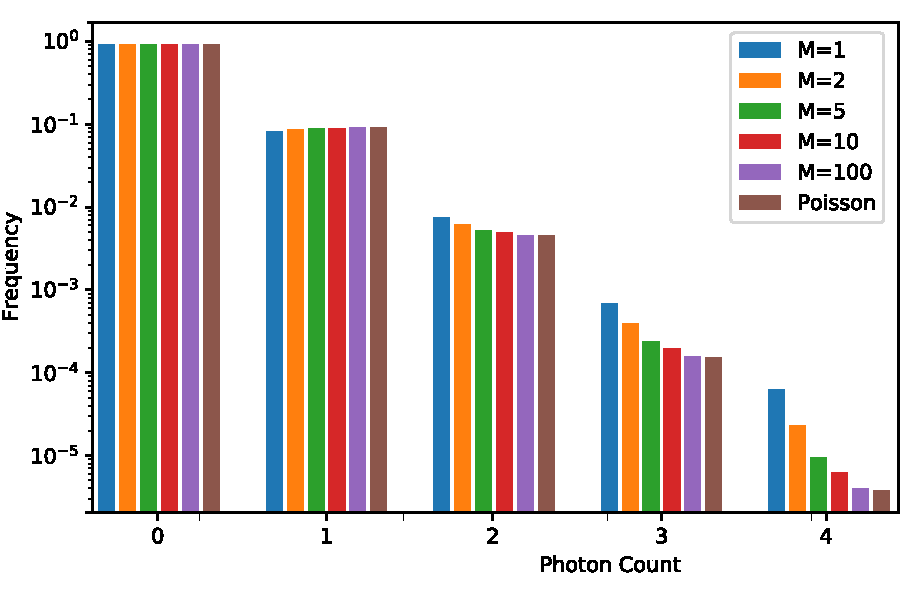
\includegraphics[width=\linewidth]{images/modes_stat.pdf}
		\caption{Photon Statistics}
		\label{fig:stat}	
		\end{subfigure}
	\caption[Temporal Modes and Photons statistics]{Temporal Modes for a Lorentzian Spectrum and Gaussian excitation (a): In the limit of longer excitation pulses, the number of modes increases linear with the pulse duration, $M\approx \frac{\text{FWHM}}{\tau_c} \sqrt{\frac{\pi} {2 \ln{2}}}$. 
		Additionally, the results of applying the mode estimation   (\fref{eq:modesp1p2}) to simulated fluorescence images as described in \fref{sec:timedependend} is shown (see there for more details on the simulation).
		
		Photon statistics with different numbers of modes $M$ and equal mean of 0.1\,photons (b): A lower number of modes corresponds the an higher probability of observing multi photon events. The limit of a high number of modes is a Poisson distribution.}
\end{figure}

The experimentally indistinguishable fluorescence energies $K_{\alpha,1}$ and $K_{\alpha,2}$ (as well as  $K_\beta$ if no filter is used for suppression) give additional independent modes $M_E$ depending on the relative intensity of the lines, with $M_E \lessapprox 2$ for the elements considered in this work (see \fref{tab:elements}).

As the used X-ray detectors are polarization insensitive and the X-ray fluorescence is unpolarized, the incoherent field can be separated into two polarization modes with independent random phase, which are pairwise orthogonal with $\vec{k}$ and therefore change slightly for each atom and detector position. For small source dimensions, this change is negligible,  giving constant $M_P \approx 2$ \cite{classen2019}. 

Path differences longer than the coherence length give additional modes $M_S$, therefore the speckle visibility will be reduced for large samples. This is for example important, if the exciting beam is not perpendicular to the detector (such as in an off-axis setup), as the excitation time difference between different parts of the a thick sample is not compensated for by the difference in flight time to the detector or in a wide angle experiment. In a small angle setup with a detector perpendicular to the beam, fluorescence from different emitters along the sample thickness will arrive at approximately equal time, hence the sample thickness should not introduce additional modes). To illustrate this effect, simulations will be performed in \fref{chap:simulation}.

If the speckle pattern is not spatially resolved by the detector because its resolution is too low compared to the change in intensity, undersampling will occur, the measured signal will be spatially averaged giving independent spatial sampling modes $M_D$ \cite{goodman2007}.

As an approximation, the total number of modes can be considered the product of those modes different numbers discussed above, even though in reality, the mode numbers are not completely independent.
Hence, in \fref{chap:simulation} simulations combining all these effects under different conditions with experimentally feasible  parameters will be performed.


\paragraph{Estimation of the Noise}
The variance of a product of (uncorrelated) photon counts following the negative binomial distribution \fref{eq:negbinomialdist} is
\begin{equation}
	\Var_{p\cdot p}= \Var_p^2 +2 \mu^2\Var_p	= \mu^4 \frac{2 M + 1}{M^2 + 2}+ \mu^3 \frac{M+1}{M} + \mu^2 \,.
\end{equation}
Assuming no correlations, this would describe the inherent noise in the measurement. The last term, dominating in the low photon count regime, can be considered as the "Poissonian character of the noise, whereas the other terms, dominating at low photon counts, the phase noise.
As shown by Trost et. al, this can be used to estimate the inherent noise of an intensity correlation measurement (up to a small term), even though the actual signal will break the assumption of having uncorrelated photon counts\cite{trost2020}.

\paragraph{Signal to Noise Ratio}
Combining the contrast of the speckle pattern, the expectation value of the product of the photon counts, the standard deviation as a quantification of the noise, and the number of independent measurements $N$ over which an average is taken, finally gives 
\begin{equation}
SNR\propto  \frac{|S(q)|^2 \mu\sqrt{N}}{M\sqrt{\mu^2 \frac{2 M + 1}{M^2 + 2}+ \mu \frac{M+1}{M} + 1}}
\end{equation}
as an estimation of the SNR, which will be further examined by performing simulations.
%Which factors influence SNR -lifetime/pulsewidth -polarisation -sampling conditions / undersampling -sample thickness / coherence length -N images -N photons

%- SNR
%will use Peak/stdev bg definition







\section{Kossel Lines}
\label{sec:kossel}
X-ray radiation  originating from \textit{within} a single crystal (such as fluorescence) can get Bragg reflected at the lattice planes of the crystal, causing Intensity variation in $90^o-\theta$ around the direction $k_{hkl}$, forming the \textit{Kossel Cones} \cite{cowley1995}. On the spherical detector centered at at the crystal, the points with influenced intensity, the \textit{Kossel lines} (or in electron microscopy more commonly \text{Kikuchi Lines}) would hence lie on circles, for a flat detector on general conic sections (see \fref{fig:kossel} for an illustration).

The visibility of the Kossel lines is governed by the same extinction rules as for the Bragg reflexes-the structure factor $F_{hkl}$ has to be non-zero. For a zinc blende structure (such as GaAs) with atomic scattering factors $f_a$ and $f_b$, the structure factor is
\begin{align}
F_{hkl} = \begin{cases}
0 & \text{if $h$, $k$, $l$ mixed parity}\\
4(f_a+f_b) & \text{if same parity and $h+k+l = 4 N$} \\
4(f_a\pm i f_b)& \text{if same parity and $h+k+l = 2 N+1$} \\
4(f_a-f_b) & \text{if same parity and $h+k+l = 4 N+2$,}
\end{cases}
\end{align}
resulting in strong Kossel lines if $h+k+l=4N$ \cite{reimer2013}.

The fine structure of the intensity variations and whether they increase or decrease the intensity over the non-scattered fluorescence background depends furthermore on the viewing direction along the cone in relation to the orientation and crystal surface \cite{faigel2016}. If the fine structure cannot be resolved by the detector and only the presence, overall shape and position of the lines is considered, no distinction between these different cases has to be explicitly made.

The Kossel lines allow to orient the detector with regards to the lattice planes. This can either be done by reprojecting the planar detector onto a sphere by an inverse gnomonic projection and determining circle center and radius, eg. by an Hugh-Transform, or by a fitting conic sections to the lines on the planar detector \cite{morris1968,morawiec2016,faigel2016,herron2018}. As the observable curvature of the Kossel lines on the detector in an IDI setup is small and therefore the circles are difficult to determine, the second method is preferable. 

As each point identified as belonging to a Kossel line has to be part of a conic section of the same plane with each cone originating from the same point, each point $r$ on a line has to fulfill

\begin{equation}
\frac{\vec{r} \cdot \vec{q}}{\left|\vec{r}\right| \left| \vec{q}\right|} = \frac{\lambda}{2d}
\end{equation}
 for a reciprocal lattice vector $\vec{q}$ which is an element of the allowed reflections $Q$. 
\begin{figure}
	\centering
	\begin{subfigure}[b]{0.3\textwidth}
	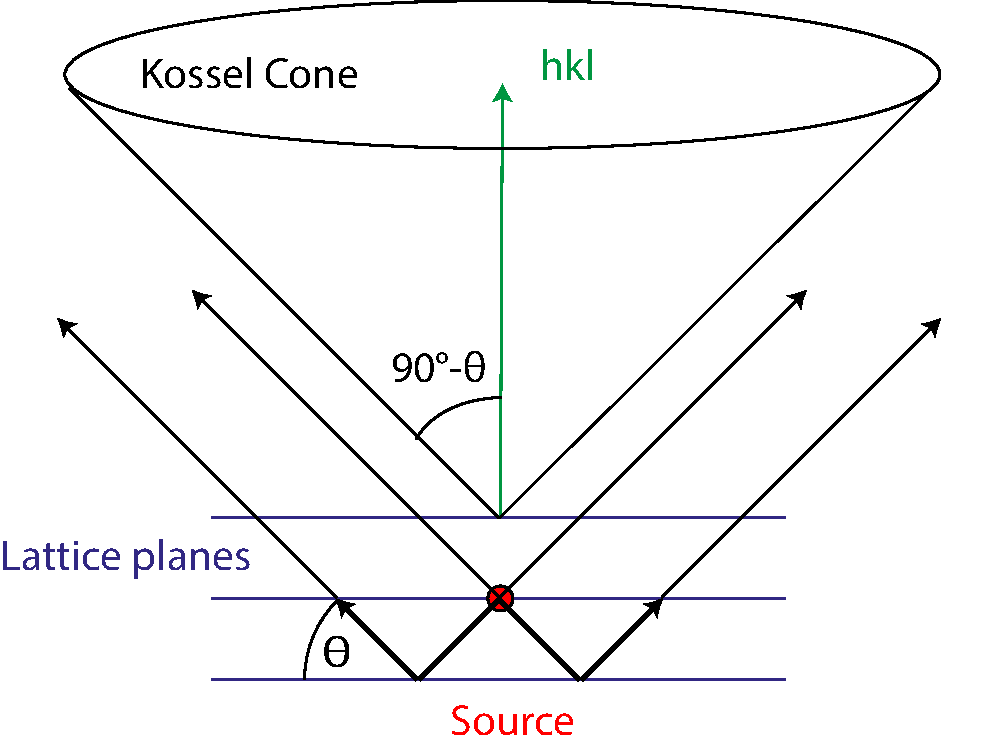
\includegraphics[width=\linewidth]{images/kossel0.pdf}
	\end{subfigure}
	\begin{subfigure}[b]{0.3\textwidth}
	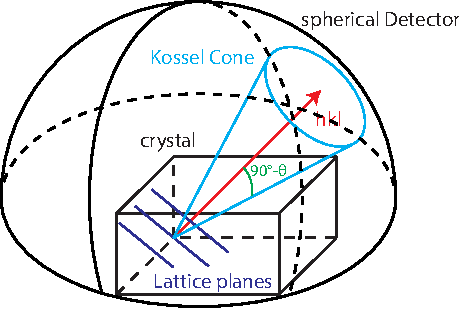
\includegraphics[width=\linewidth]{images/kossel.pdf}
	\end{subfigure}
	\begin{subfigure}[b]{0.35\textwidth}
	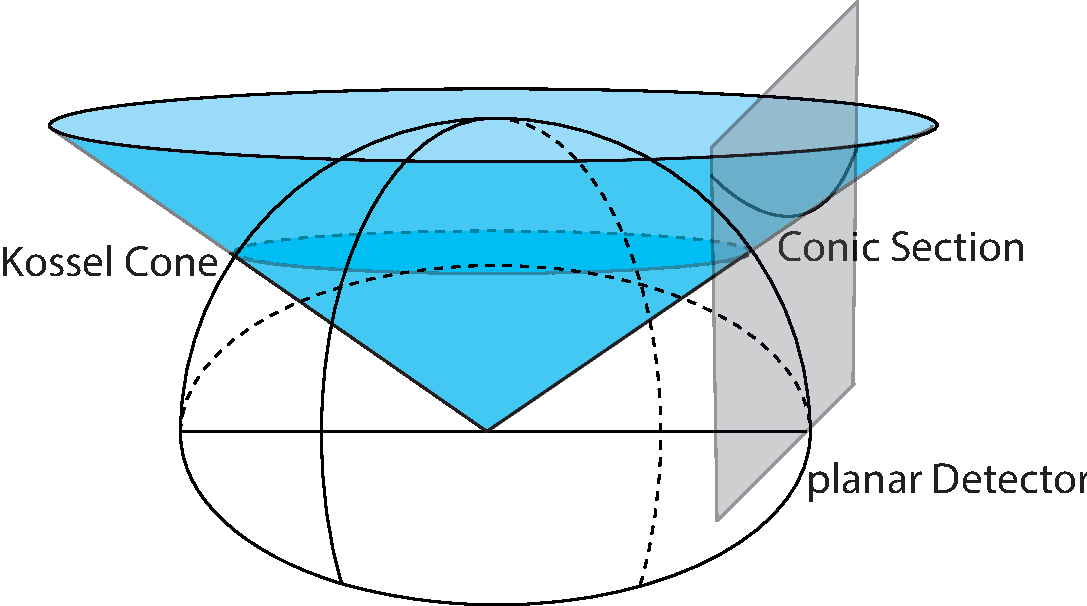
\includegraphics[width=\linewidth]{images/kossel2.pdf}
	\end{subfigure}
	\caption[Geometry of Kossel Lines]{Geometry of Kossel Lines: Radiation from within a light source within a single crystal gets scattered at the lattice planes, causing a change in intensity along a cone of opening angle $90^o-\theta_{hkl}$ and vertex hkl (left). On a spherical detector centered around the sample, those intensity changes would be visible as circular Kossel lines (center). On a planar detector, the intersections of the Kossel cones are visible as conic sections (right)}
	\label{fig:kossel}
\end{figure}
